% Source: graduate-coursework/Sp26/CSCE775/course_notes/mc_action_values_guide.tex

\documentclass[border=4pt]{standalone}
\usepackage{amsfonts}
\usepackage{amsmath}
\usepackage{amssymb}
\usepackage{amsthm}
\usepackage[T1]{fontenc}
\usepackage{graphicx}
\usepackage{tikz}
\usepackage{xcolor}
\usetikzlibrary{arrows.meta, positioning, shapes.geometric, calc, decorations.pathreplacing}

\definecolor{Garnet}{HTML}{73000a}
\definecolor{SecondaryBlue}{HTML}{466A9F}
\definecolor{SecondaryGreen}{HTML}{65780B}
\definecolor{FlatRed}{HTML}{CC2E40}
\definecolor{FlatDark}{HTML}{1F414D}
\definecolor{FlatYellow}{HTML}{CED318}
\definecolor{FlatGold}{HTML}{A49137}
\definecolor{LightGray}{HTML}{F0F0F0}
\definecolor{Rose}{HTML}{CC2E40}

\renewcommand{\baselinestretch}{1.2}
\newcommand{\vocab}[1]{\textbf{\textcolor{Garnet}{#1}}}
\newcommand{\mathhighlight}[1]{\textcolor{SecondaryBlue}{#1}}

\begin{document}
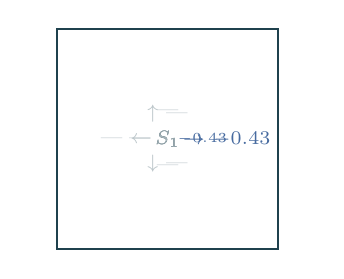
\begin{tikzpicture}[
    cell/.style={minimum size=2.8cm, draw=FlatDark, thick},
    goal/.style={cell, fill=Garnet!15, draw=Garnet, line width=1.5pt},
    qval/.style={font=\scriptsize\bfseries, SecondaryBlue},
    qempty/.style={font=\scriptsize, FlatDark!30},
    slabel/.style={font=\scriptsize, FlatDark}
]
% Helper macro for Q-cell contents
% Arguments: node name, Up val, Down val, Left val, Right val
% --- S1 ---
\node[cell] (s1) at (0, 5.6) {};
\node[slabel] at ([shift={(0,0)}]s1.center) {$S_1$};
\node[qempty] at ([yshift=10pt]s1.center) {---};   % Up
\node[qempty] at ([yshift=-10pt]s1.center) {---};  % Down
\node[qempty] at ([xshift=-10pt]s1.center) {---};  % Left
\node[qval] at ([xshift=10pt, yshift=0pt]s1.east) {};
\node[qval, anchor=west] at ([xshift=0pt]s1.center) {\tiny $-0.43$};

% Redraw S1 with proper layout
\begin{scope}
\node[cell] (c1) at (0, 5.6) {};
\node[slabel, anchor=center] at (c1.center) {\textcolor{FlatDark!40}{$S_1$}};
\node[qempty] at ([yshift=9pt]c1.center) {$\uparrow$ ---};
\node[qempty] at ([yshift=-9pt]c1.center) {$\downarrow$ ---};
\node[qempty] at ([xshift=-7pt, yshift=0pt]c1.west) {};
\node[font=\scriptsize, FlatDark!30, anchor=east] at ([xshift=-2pt]c1.center) {--- $\leftarrow$};
\node[qval, anchor=west] at ([xshift=2pt]c1.center) {$\rightarrow$ $-0.43$};
\end{scope}
\end{tikzpicture}
\end{document}
